\subsection*{Question 4}

\textbf{a)} Answer the same question as in Q3 using a Metropolis algorithm with vector proposals for $\bm{\theta}$ and making use of the variance-covariance matrix from the Laplace approximation in Q2d. Use the same number of iterations (after burnin) as in Q3.

\begin{center}\rule{6cm}{0.4pt}\end{center}

In order to get $\SI{20}{\percent}$ of acceptance rate, we multiplied the variance obtained from the variance-covariance matrix by a factor of $20$.

\begin{figure}[H]
	\centering
	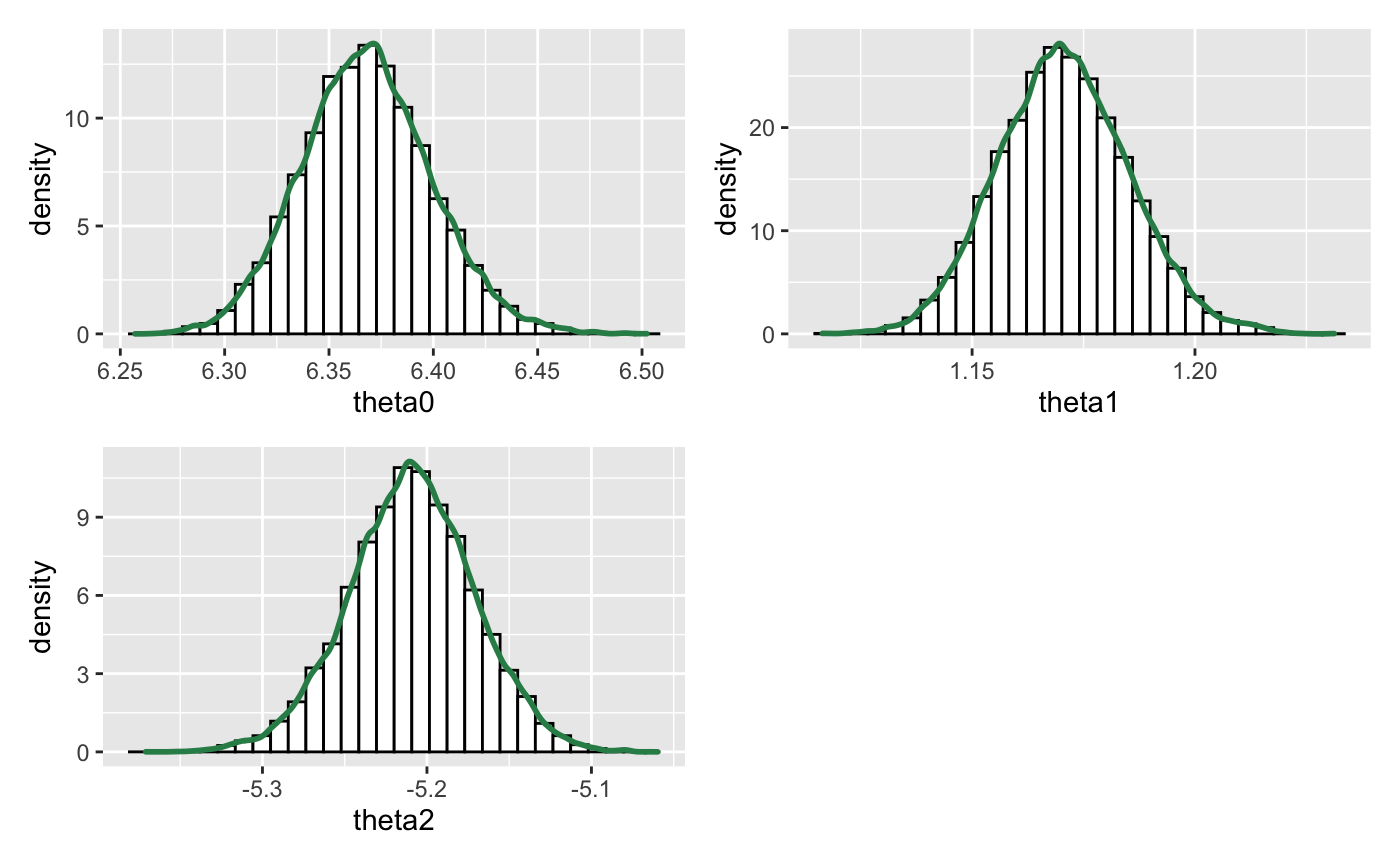
\includegraphics[width=0.7\textwidth]{figures/metropolis_vw/metropolis_vw_samples.png}
	\caption{Random sample from the posterior distribution of $(\vec{\theta}|\mathcal{D}_1)$ using a vector-wise metropolis algorithm}
	\label{fig:metropolis_vw_samples}
\end{figure}

\subsubsection*{Convergence}

From the visual analysis, we have a good mixing which is a good signal of convergence.

\begin{figure}[H]
	\centering
	\begin{subfigure}{0.3\textwidth}
		\centering
		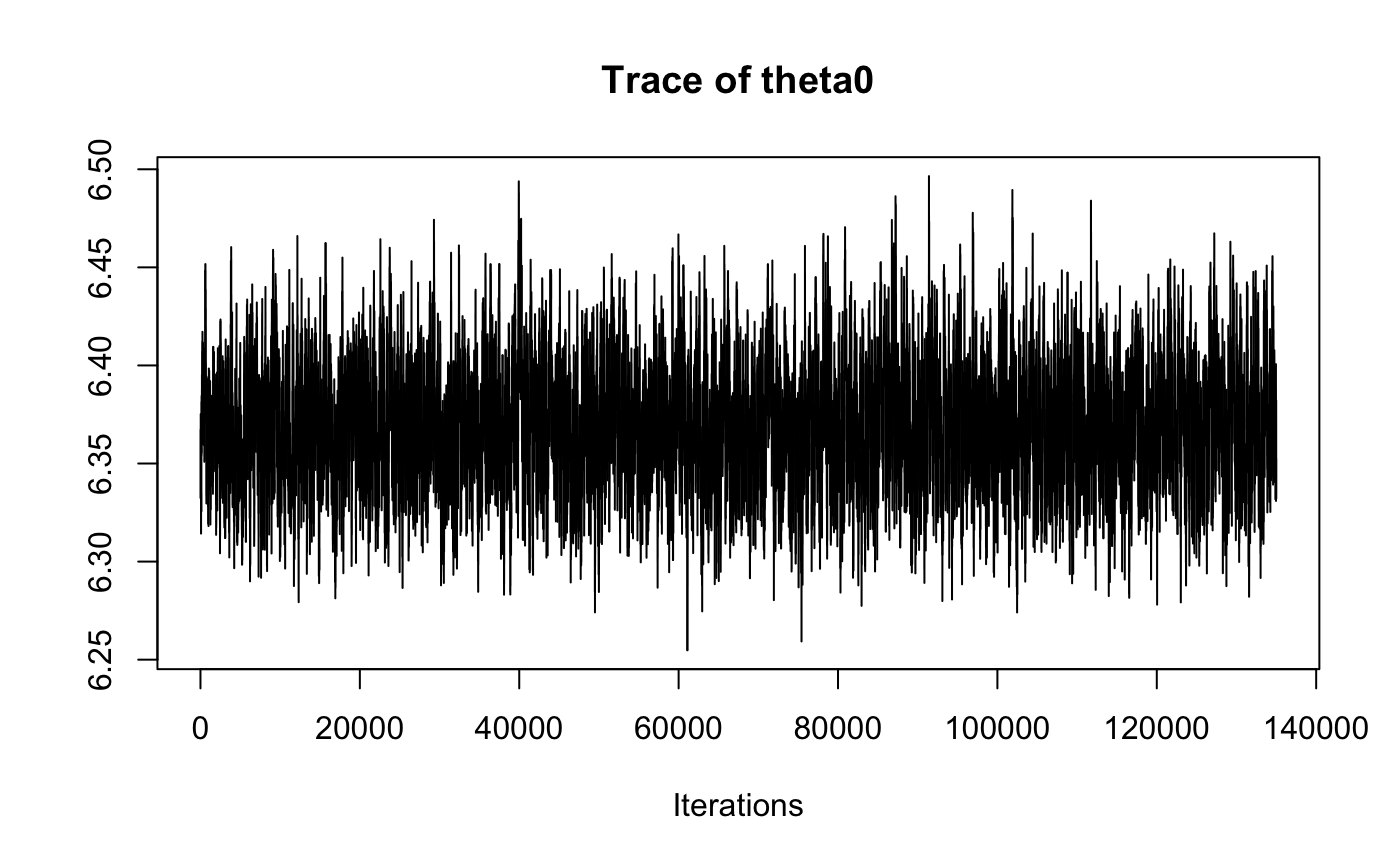
\includegraphics{figures/metropolis_vw/metropolis_vw_traceplot_theta0}
	\end{subfigure}
	\begin{subfigure}{0.3\textwidth}
		\centering
		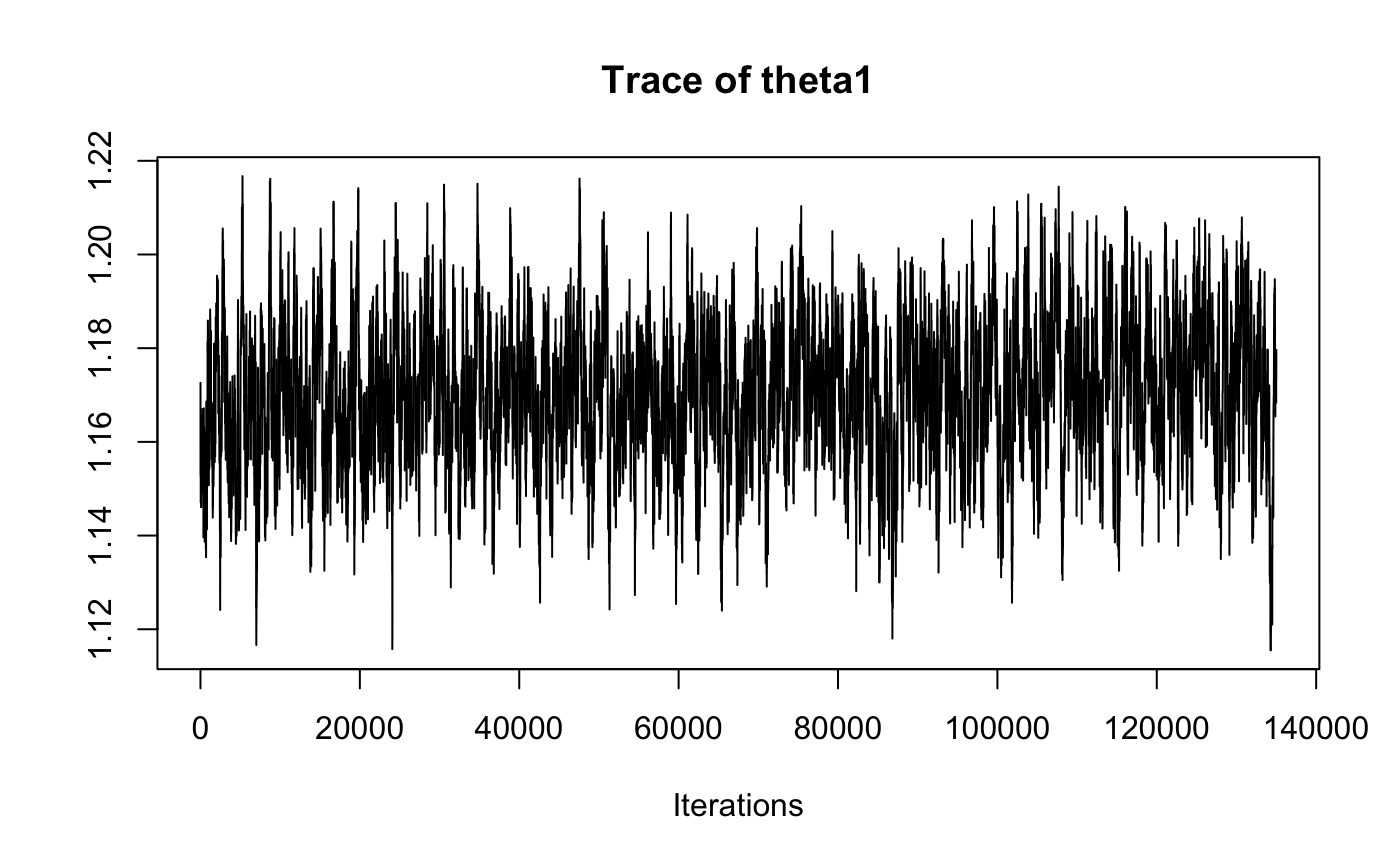
\includegraphics{figures/metropolis_vw/metropolis_vw_traceplot_theta1}
	\end{subfigure}
	\begin{subfigure}{0.3\textwidth}
		\centering
		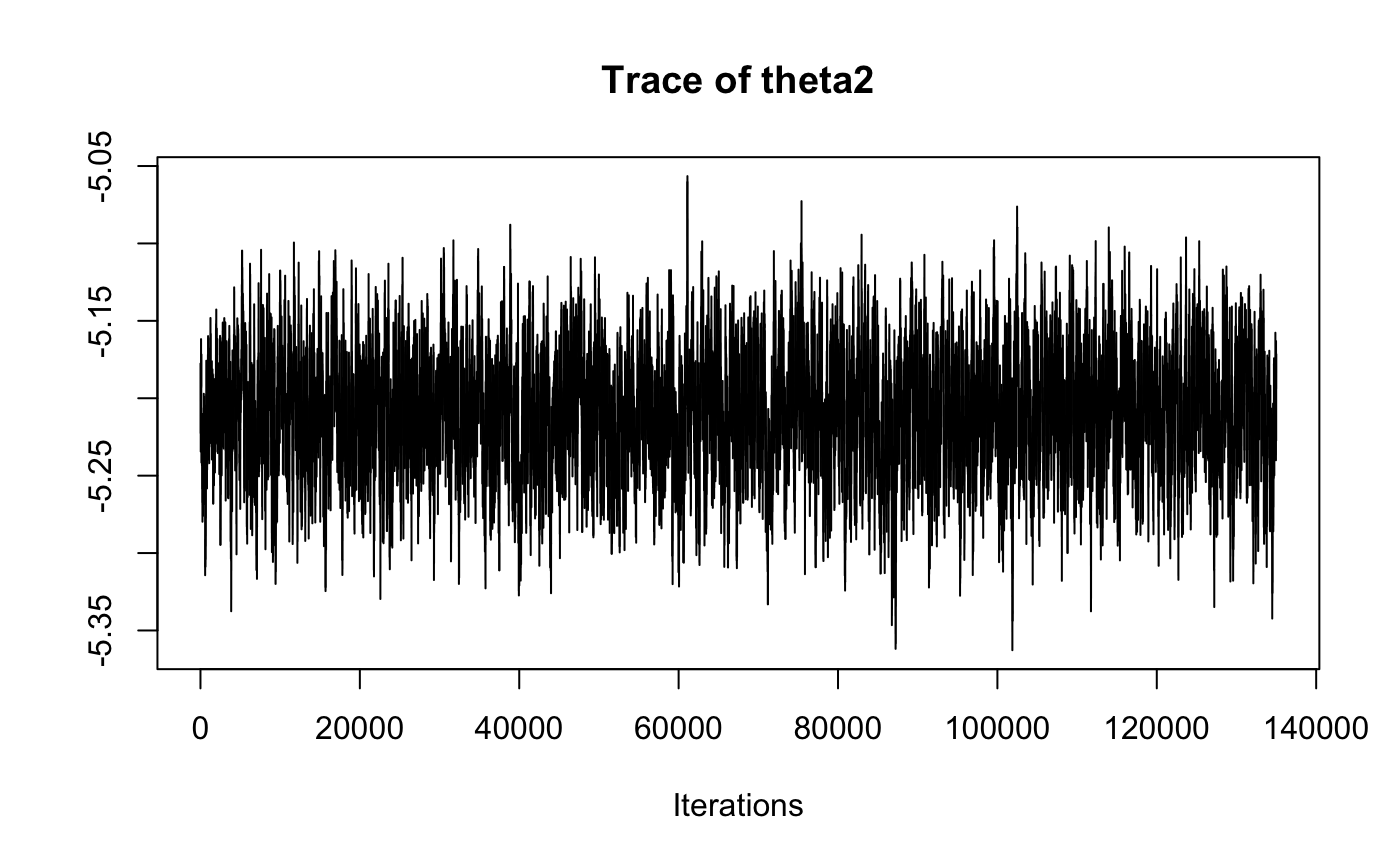
\includegraphics{figures/metropolis_vw/metropolis_vw_traceplot_theta2}
	\end{subfigure}
	\caption{Traceplots of the $\theta_k$ parameters}
	\label{fig:metropolis-vw-traceplots}
\end{figure}

Moreover, the $\hat{R}$ computed from the Gelman statistic is below $1.1$ and we notice from the Geweke test that at a $\SI{5}{\percent}$ significance level, we cannot reject the null hypothesis that the mean of the two computed subchains are equal for each parameter. Therefore we have a strong confidence in the convergence of the metropolis vector-wise algorithm.

\begin{table}[H]
	\centering\begin{tabular}{|c|c|c|} \hline 
		parameters & $\hat{R}$ & upper C.I. \\ \hline
		$\theta_0$ & $1.000513$ & $1.000901$ \\
		$\theta_1$ & $1.001974$ & $1.002180$ \\
		$\theta_2$ & $1.000653$ & $1.001020$ \\ \hline
	\end{tabular}
	\caption{Results of the Gelbman-Rubin test}
	\label{tab:metropolis-vw-gelman-rubin}
\end{table}

\begin{table}[H]
	\centering\begin{tabular}{|c|c|c|} \hline 
		parameters & z-score & p-value \\ \hline
		$\theta_0$ & $-0.4956$ & $0.6899117$ \\
		$\theta_1$ & $-1.7949$ & $0.9636652$ \\
		$\theta_2$ & $-0.4138$ & $0.6604897$ \\ \hline
	\end{tabular}
	\caption{Results for the Geweke statistic (z-score)}
	\label{tab:metropolis-cw-geweke}
\end{table}

Finally, we have at least $500$ effective samples for each parameter.

\begin{table}[H]
	\centering\begin{tabular}{|c|c|c|} \hline 
		$\theta_0$ & $\theta_1$ & $\theta_2$ \\ \hline 
		$1682.979$  & $504.130$ & $1282.254$   \\ \hline
	\end{tabular}
	\caption{Effective sample sizes}
	\label{tab:metropolis-vw-effective-sample-sizes}
\end{table}

\textbf{b)} Compare your results with the previous ones.

\begin{center}\rule{6cm}{0.4pt}\end{center}

\subsubsection*{Fitted curve}

The mean for each $\bm{\theta}$ parameter is the same as for the component-wise algorithm. Therefore, as expected, the growth rate of cancer cells is again underestimate by our model.

\begin{figure}[H]
	\centering
	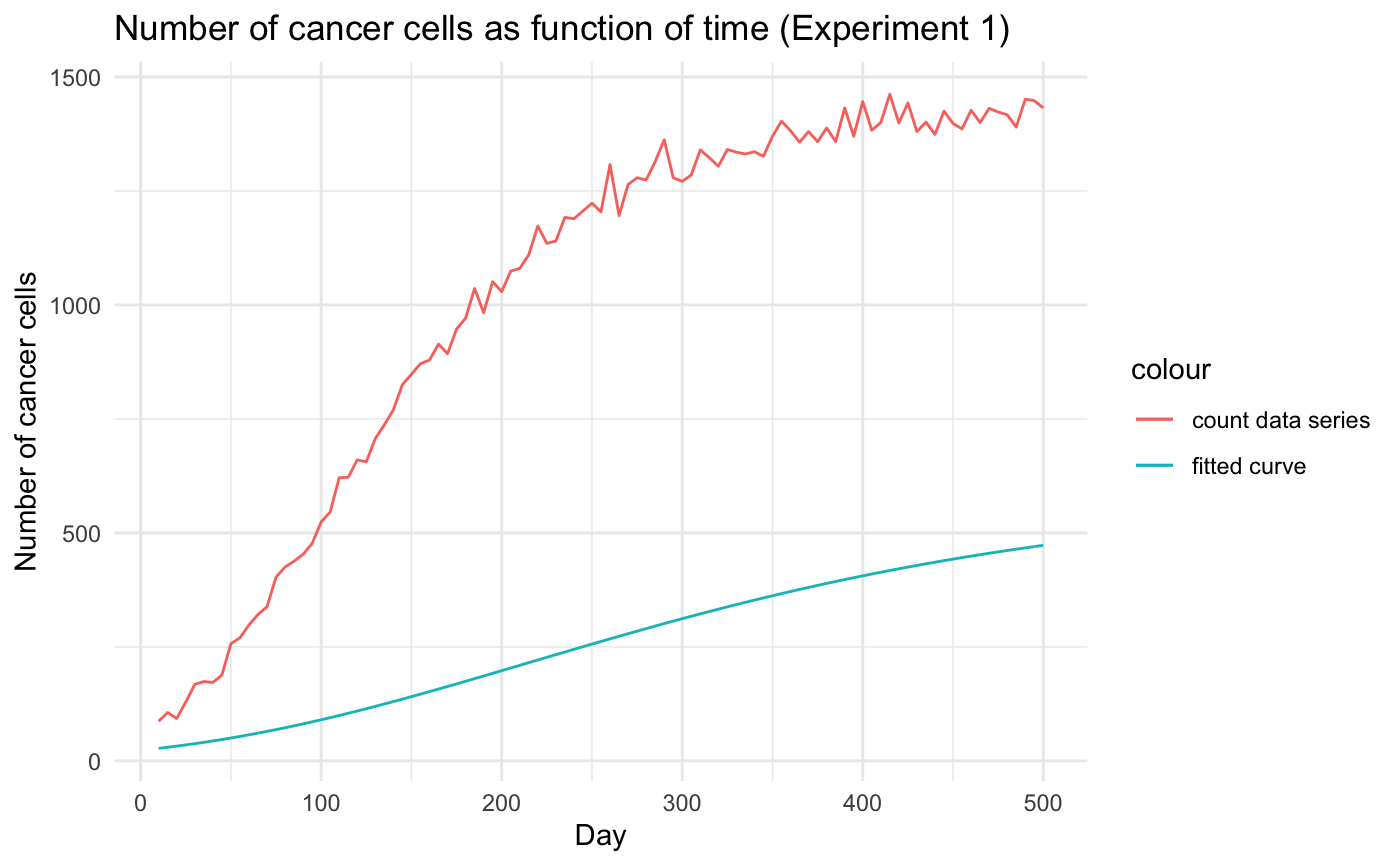
\includegraphics[width=0.7\textwidth]{figures/metropolis_vw/metropolis_vw_fitted_curve.png}
	\caption{Comparison of the observed count data series for experiment 1 (\textit{black}) with the fitted curve for $\mu(t)$ (\textit{red})}
	\label{fig:metropolis-vw-fitted-curve}
\end{figure}

\subsubsection*{Point estimate and $\SI{95}{\percent}$ credible region}

Following what we said above, obviously we get the point estimate and credible regions for the $\bm{\beta}$ parameters.

\begin{table}[H]
	\centering\begin{tabular}{|c|c|c|} \hline 
		Parameter & Median & Mean \\ \hline 
		$\theta_0$ & $6.37$ & $6.37$ \\ 
		$\theta_1$ & $1.17$ & $1.17$ \\
		$\theta_2$ & $-5.21$ & $-5.21$ \\ \hline
	\end{tabular}
	\caption{Point estimates of $\bm{\theta}$ parameters}
	\label{tab:metropolis-cw-point-estimates}
\end{table}

\begin{table}[H]
	\centering\begin{tabular}{|c|c|c|} \hline 
		Parameter & Lower & Upper \\ \hline 
		$\theta_0$ & $6.31$ & $6.42$ \\ 
		$\theta_1$ & $1.14$ & $1.19$ \\
		$\theta_2$ & $-5.28$ & $-5.13$ \\ \hline
	\end{tabular}
	\caption{$\SI{95}{\percent}$ credible region for $\bm{\theta}$ parameters}
	\label{tab:metropolis-cw-credible-region}
\end{table}